\documentclass{article}
% Change "article" to "report" to get rid of page number on title page
\usepackage{amsmath,amsfonts,amsthm,amssymb}
\usepackage{setspace}
\usepackage{Tabbing}
\usepackage{fancyhdr}
\usepackage{lastpage}
\usepackage{extramarks}
\usepackage{chngpage}
\usepackage{soul,color}
\usepackage{graphicx,float,wrapfig}
\usepackage{multirow}
\usepackage{enumerate}
 \usepackage[hang,small]{caption}
% In case you need to adjust margins:
\topmargin=-0.45in      %
\evensidemargin=0in     %
\oddsidemargin=0in      %
\textwidth=6.5in        %
\textheight=9.0in       %
\headsep=0.25in         %

% Homework Specific Information
\newcommand{\hmwkTitle}{The Fall of Gibbs Sampling}
\newcommand{\hmwkClass}{}
\newcommand{\hmwkAuthorName}{Donglai\ Wei}


% Setup the header and footer
\pagestyle{fancy}                                                       %
\lhead{\hmwkAuthorName}                                                 %
\rhead{\firstxmark}                                                     %
\lfoot{\lastxmark}                                                      %
\cfoot{}                                                                %
\rfoot{Page\ \thepage\ of\ \pageref{LastPage}}                          %
\renewcommand\headrulewidth{0.4pt}                                      %
\renewcommand\footrulewidth{0.4pt}                                      %

% This is used to trace down (pin point) problems
% in latexing a document:
%\tracingall

%%%%%%%%%%%%%%%%%%%%%%%%%%%%%%%%%%%%%%%%%%%%%%%%%%%%%%%%\begin{enumerate}

% Some tools
\newcommand{\enterProblemHeader}[1]{\nobreak\extramarks{#1}{#1 continued on next page\ldots}\nobreak%
                                    \nobreak\extramarks{#1 (continued)}{#1 continued on next page\ldots}\nobreak}%
\newcommand{\exitProblemHeader}[1]{\nobreak\extramarks{#1 (continued)}{#1 continued on next page\ldots}\nobreak%
                                   \nobreak\extramarks{#1}{}\nobreak}%

\newlength{\labelLength}
\newcommand{\labelAnswer}[2]
  {\settowidth{\labelLength}{#1}%
   \addtolength{\labelLength}{0.25in}%
   \changetext{}{-\labelLength}{}{}{}%
   \noindent\fbox{\begin{minipage}[c]{\columnwidth}#2\end{minipage}}%
   \marginpar{\fbox{#1}}%

   % We put the blank space above in order to make sure this
   % \marginpar gets correctly placed.
   \changetext{}{+\labelLength}{}{}{}}%

\setcounter{secnumdepth}{0}
\newcommand{\homeworkProblemName}{}%
\newcounter{homeworkProblemCounter}%
\newenvironment{homeworkProblem}[1][Problem \arabic{homeworkProblemCounter}]%
  {\stepcounter{homeworkProblemCounter}%
   \renewcommand{\homeworkProblemName}{#1}%
   \section{\homeworkProblemName}%
   \enterProblemHeader{\homeworkProblemName}}%
  {\exitProblemHeader{\homeworkProblemName}}%

\newcommand{\problemAnswer}[1]
  {\noindent\fbox{\begin{minipage}[c]{\columnwidth}#1\end{minipage}}}%

\newcommand{\problemLAnswer}[1]
  {\labelAnswer{\homeworkProblemName}{#1}}

\newcommand{\homeworkSectionName}{}%
\newlength{\homeworkSectionLabelLength}{}%
\newenvironment{homeworkSection}[1]%
  {% We put this space here to make sure we're not connected to the above.
   % Otherwise the changetext can do funny things to the other margin

   \renewcommand{\homeworkSectionName}{#1}%
   \settowidth{\homeworkSectionLabelLength}{\homeworkSectionName}%
   \addtolength{\homeworkSectionLabelLength}{0.25in}%
   \changetext{}{-\homeworkSectionLabelLength}{}{}{}%
   \subsection{\homeworkSectionName}%
   \enterProblemHeader{\homeworkProblemName\ [\homeworkSectionName]}}%
  {\enterProblemHeader{\homeworkProblemName}%

   % We put the blank space above in order to make sure this margin
   % change doesn't happen too soon (otherwise \sectionAnswer's can
   % get ugly about their \marginpar placement.
   \changetext{}{+\homeworkSectionLabelLength}{}{}{}}%

\newcommand{\sectionAnswer}[1]
  {% We put this space here to make sure we're disconnected from the previous
   % passage

   \noindent\fbox{\begin{minipage}[c]{\columnwidth}#1\end{minipage}}%
   \enterProblemHeader{\homeworkProblemName}\exitProblemHeader{\homeworkProblemName}%
   \marginpar{\fbox{\homeworkSectionName}}%

   % We put the blank space above in order to make sure this
   % \marginpar gets correctly placed.
   }%

%%%%%%%%%%%%%%%%%%%%%%%%%%%%%%%%%%%%%%%%%%%%%%%%%%%%%%%%%%%%%



%%%%%%%%%%%%%%%%%%%%%%%%%%%%%%%%%%%%%%%%%%%%%%%%%%%%%%%%%%%%%
% Make title
\title{\vspace{0.3in}\textmd{\textbf{\hmwkTitle}}}
\date{2010.6.1}
\author{\textbf{\hmwkAuthorName}}
%%%%%%%%%%%%%%%%%%%%%%%%%%%%%%%%%%%%%%%%%%%%%%%%%%%%%%%%%%%%%

\begin{document}
\begin{spacing}{1.1}
\maketitle

\section{0) Expectation}
Thought Gibbs sampling works better than ME search on the small set of data(40 restaurants,5*5,10 bars), we expect for a larger data set
(1000 restaurants,5*5,10 bars):\\ \\
1)Gibbs Sampling will have a hard time jumping out of the local maxima\\ \\
2)The Split move in ME search will instead benefit from the information shared across more restaurants\\

\section{1) Experiment}
1000 restaurants,5*5,10 bars\\

\subsection{i) Ground Truth}
\begin{figure}[h] 
  \begin{minipage}[b]{0.5\textwidth} 
    \centering 
    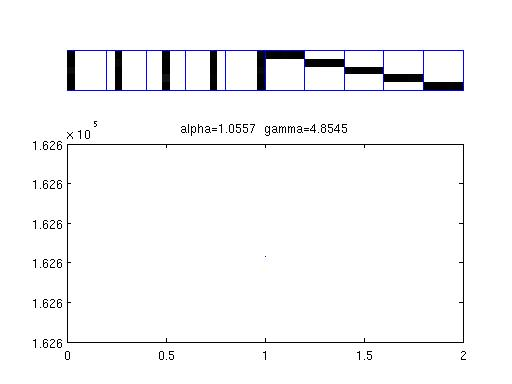
\includegraphics[width=2.5in,height=2in]{gt.jpg} 
    \caption{Ground Truth:Table Config for the first 40 restaurants}
    \label{fig:by:table} 
  \end{minipage}% 
  \begin{minipage}[b]{0.5\textwidth} 
    \centering 
    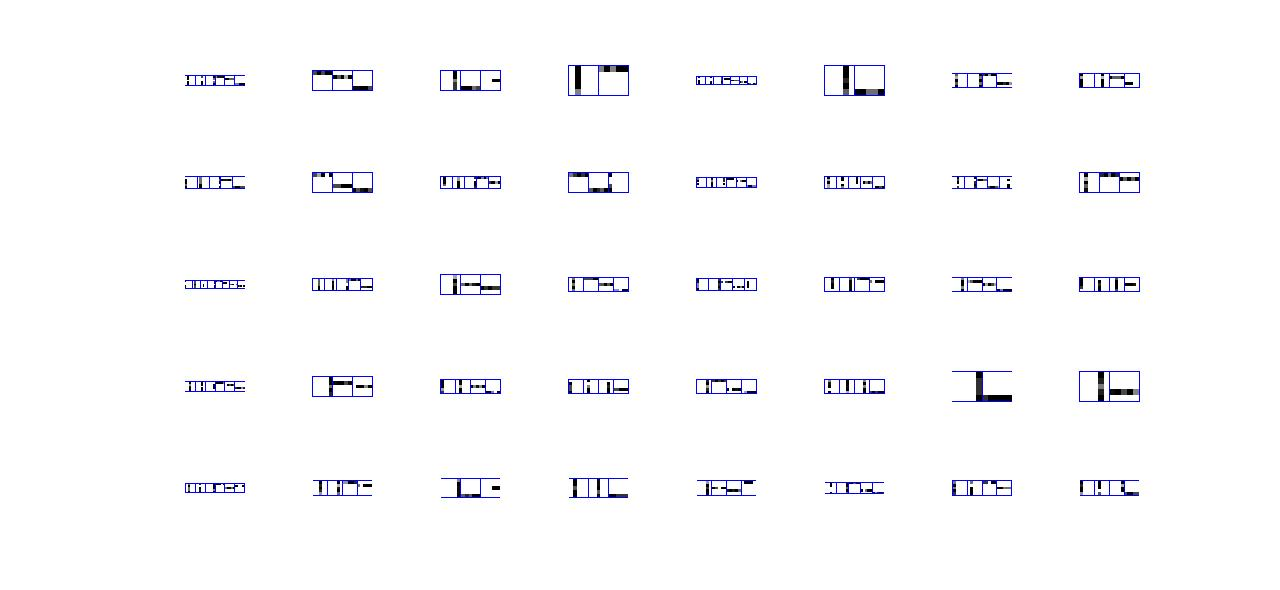
\includegraphics[width=2.5in,height=2in]{g_td.jpg} 
    \caption{Ground Truth:Dish Config and -log Probability}
    \label{fig:by:table}  
   \end{minipage}% 
\end{figure}

\subsection{ii) Gibbs Sampling}
\begin{figure}[h] 
  \begin{minipage}[b]{0.5\textwidth} 
    \centering 
    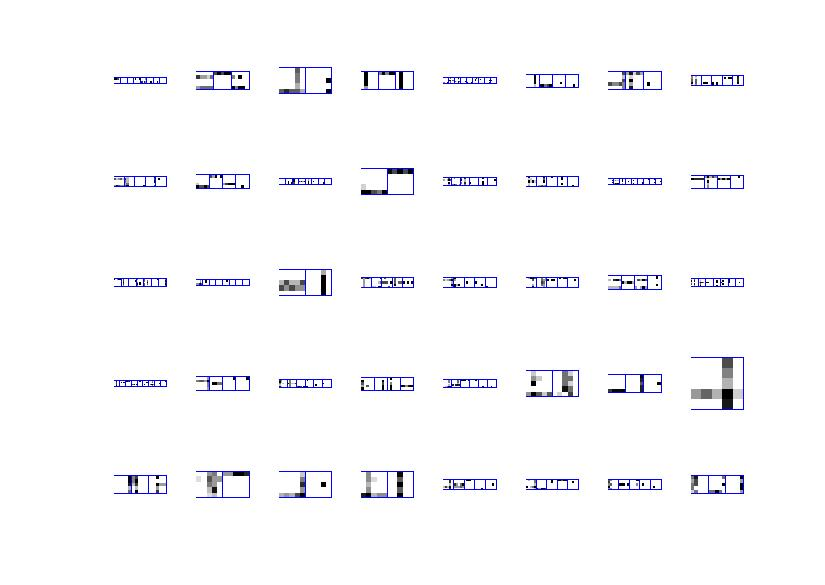
\includegraphics[width=2.5in,height=2in]{Gobbs1000d.jpg} 
    \caption{Gibbs Sampling:Table Config for the first 40 restaurants}
    \label{fig:by:table} 
  \end{minipage}% 
  \begin{minipage}[b]{0.5\textwidth} 
    \centering 
    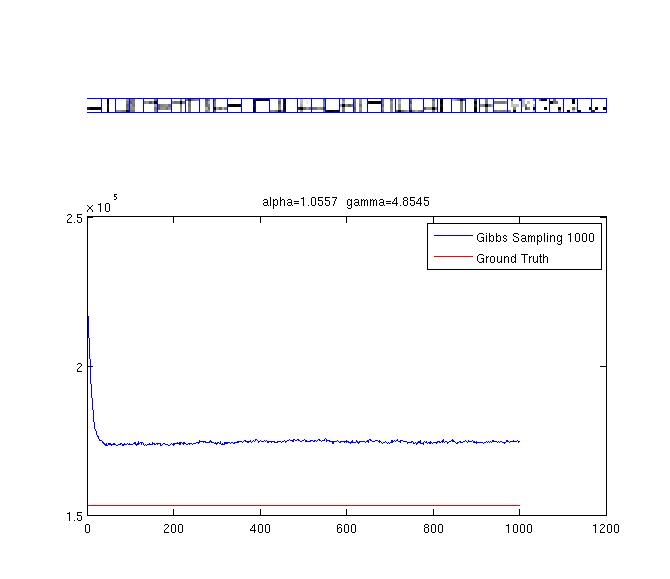
\includegraphics[width=2.5in,height=2in]{g_t.jpg} 
    \caption{Gibbs Sampling:Dish Config and -log Probability}
    \label{fig:by:table}  
   \end{minipage}% 
\end{figure}


\subsection{iii) ME search after Ground Truth and Gibbs Sampling}
\begin{figure}[h] 
  \begin{minipage}[b]{0.5\textwidth} 
    \centering 
    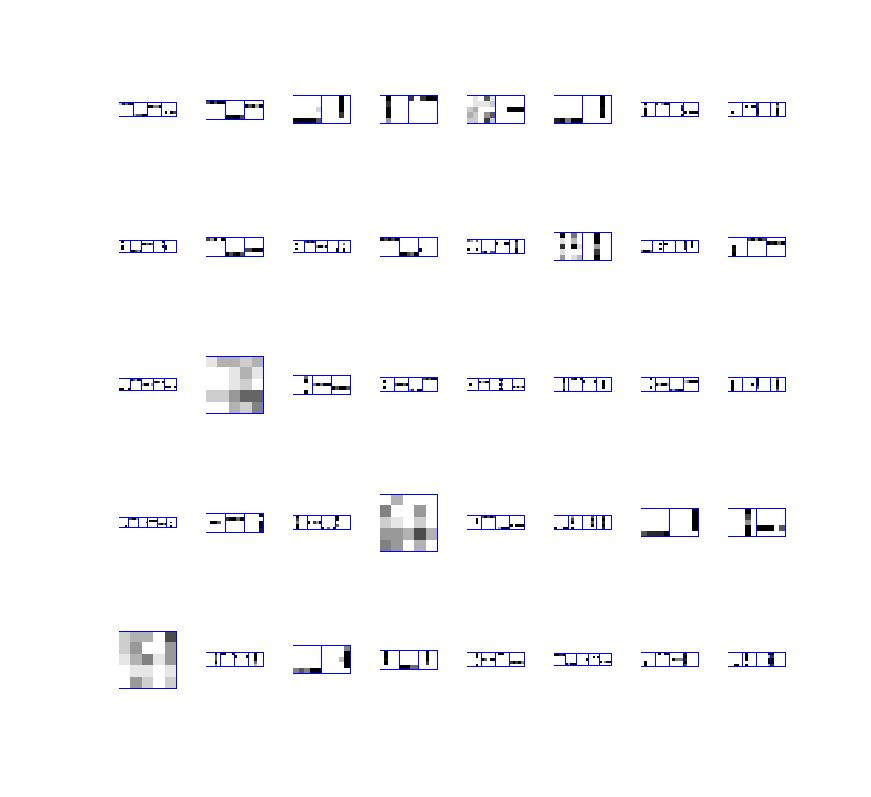
\includegraphics[width=2.5in,height=2in]{g_t_me1.jpg} 
    \caption{ME after Ground Truth:Table Config for the first 40 restaurants}
    \label{fig:by:table} 
  \end{minipage}% 
  \begin{minipage}[b]{0.5\textwidth} 
    \centering 
    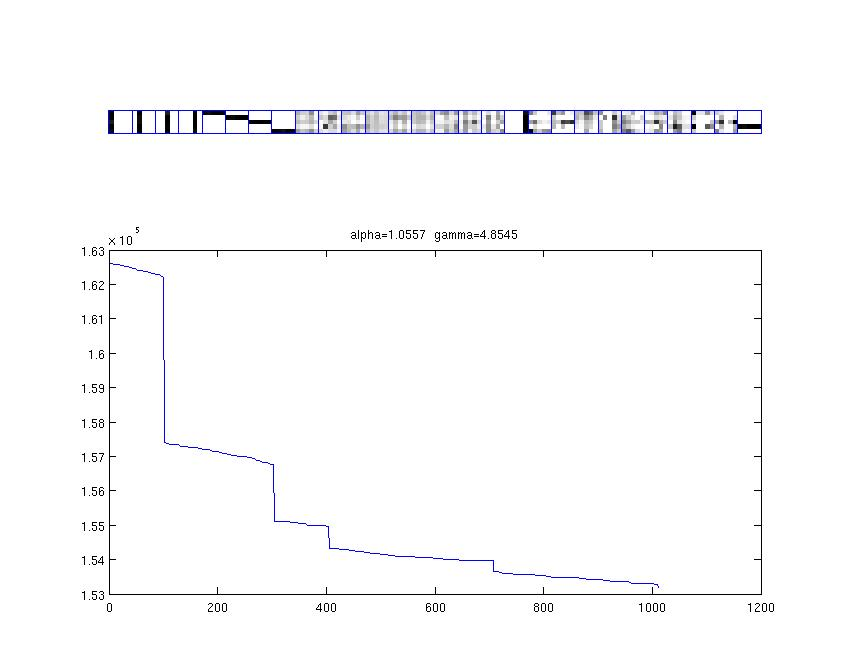
\includegraphics[width=2.5in,height=2in]{g_t_me1d.jpg} 
    \caption{ME after Ground Truth:Dish Config and -log Probability}
    \label{fig:by:table}  
   \end{minipage}% 
\end{figure}
\begin{figure}[h] 
  \begin{minipage}[b]{0.5\textwidth} 
    \centering 
    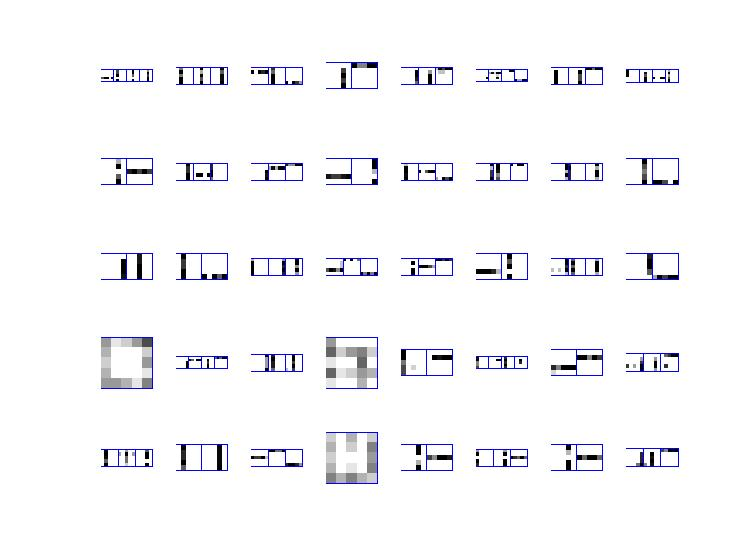
\includegraphics[width=2.5in,height=2in]{init1_5_nmt85_allll.jpg} 
    \caption{ME after Gibbs Sampling:Table Config for the first 40 restaurants}
    \label{fig:by:table} 
  \end{minipage}% 
  \begin{minipage}[b]{0.5\textwidth} 
    \centering 
    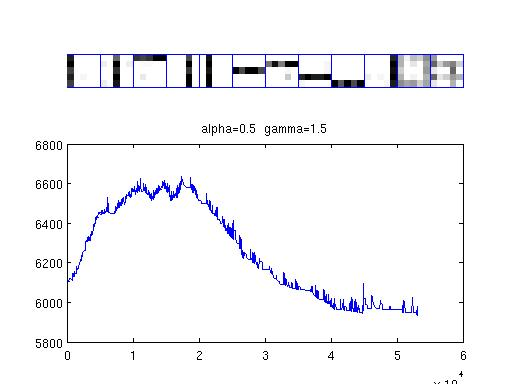
\includegraphics[width=2.5in,height=2in]{init1_5_nmt85_allll_d.jpg} 
    \caption{ME after Gibbs Sampling:Dish Config and -log Probability}
    \label{fig:by:table}  
   \end{minipage}% 
\end{figure}


\end{spacing}
\end{document}

%%%%%%%%%%%%%%%%%%%%%%%%%%%%%%%%%%%%%%%%%%%%%%%%%%%%%%%%%%%%%
